\section{Задание 3. Интегралы Пуассона и Френеля}

\textbf{Условие.}

Вычислите интеграл $K$:

\[\int_0^{+\infty} \frac{\sin\left(\frac{\pi}{2} - t\right)}{\sqrt{t}} dt\]

Замечание. В задачах физики и дифракционной оптики возникают интегралы вида:

\[\int e^{-x^2} dx, \int \frac{\sin(t)}{\sqrt{t}} dt, \int \frac{\cos(t)}{\sqrt{t}} dt\]

которые являются специальными функциями (т.е. \enquote{неберущимися} интегралами).

Однако, переход к \enquote{многомерным} интегралам позволяет вычислить по крайней мере функцию ошибок
$\Phi(z) = \int_0^z e^{-x^2} dx$ и интегралы Френеля: $\Phi_S(z) = \int_0^z \frac{\sin(t)}{\sqrt{t}} dt$ и $\Phi_C(z) = \int_0^z \frac{\cos(t)}{\sqrt{t}} dt$

\begin{enumerate}
    \item Вычисление $\int^{+\infty}_0 e^{-x^2} dx = I$:
    \begin{itemize}
        \item Заметьте, что $\displaystyle I = \int^{+\infty}_0 e^{-x^2} dx = \int_0^{+\infty} e^{-y^2} dy$
        Тогда $\displaystyle I^2 = \int^{+\infty}_0 e^{-x^2} dx \int_0^{+\infty} e^{-y^2} dy$ - двукратный интеграл.

        \item Перейдите к полярным координатам и вычислите его.
    \end{itemize}

    \item Вычисление $\displaystyle \int_0^{+\infty} \frac{\cos(t)}{\sqrt{t}} dt = J$
    \begin{itemize}
        \item Используя результат пункта 1), докажите справедливость интегрального представления функции
        $\displaystyle \frac{2}{\sqrt{\pi}} \int_0^{+\infty} e^{-u^2 t} du = \frac{1}{\sqrt{t}}$.В интеграле $J$ замените функцию $\frac{1}{\sqrt{t}}$ её интегральным представлением и получите двойной (несобственный) интеграл.

        \item Выберите порядок интегрирования так, чтобы можно было найти первообразную в элементарных функциях.
        (Смена порядка интегрирования требует обоснования, но в данном случае она разрешена.)

        \item Вычислите интеграл $J$, затем интеграл $K$.

        \item Используя замену переменной и сводя эти интегралы к $J$, вычислите также:

        $\displaystyle \int_0^{+\infty} \cos(x^2) dx$ и $\displaystyle \int_0^{+\infty} \cos(\frac{\pi x^2}{2}) dx$

    \end{itemize}

    \item Нарисуйте графики функции ошибок, интегралов Френеля и их подынтегральных функций.

\end{enumerate}

\vspace{10mm}
\textbf{Решение.}

\begin{enumerate}
    \item
        Полярные координаты:
        \begin{equation}
            \begin{cases}
                x = \cos\varphi \cdot \rho \\
                y = \sin\varphi \cdot r
            \end{cases}
        \end{equation}
        Ограничения на $x$, $y$:
        \begin{equation}
            \begin{cases}
                0 \leq x < {+\infty} \\
                0 \leq y < {+\infty}
            \end{cases}
        \end{equation}
        Т. е. мы ограничены первой четвертью пространства. Рассмотрим это в полярных координатах: 
        \begin{equation}
            \begin{cases}
                0 \leq \varphi \leq \frac{\pi}{2} \\
                0 \leq \rho < {+\infty}
            \end{cases}
        \end{equation}
        Найдём Якобиану перевода из ДПСК в ПСК:
        $\displaystyle J = \begin{matrix}
            \frac{\partial x}{\partial \rho} & \frac{\partial x}{\partial \varphi} \\
            \frac{\partial y}{\partial \rho} & \frac{\partial y}{\partial \varphi}
        \end{matrix} = 
        \begin{matrix}
            \frac{\partial (\cos\varphi \cdot \rho)}{\partial \rho} & \frac{\partial (\cos\varphi \cdot \rho)}{\partial \varphi} \\
            \frac{\partial (\sin\varphi \cdot \rho)}{\partial \rho} & \frac{\partial (\sin\varphi \cdot \rho)}{\partial \varphi}
        \end{matrix} =
        \begin{matrix}
            \cos\varphi & -\sin\varphi \cdot \rho \\
            \sin\varphi & \cos\varphi \cdot \rho
        \end{matrix} =
        \rho \begin{matrix}
            \cos\varphi & -\sin\varphi \\
            \sin\varphi & \cos\varphi 
        \end{matrix} = \rho$

        Преобразуем двойной интеграл в ПСК: \\
        $\displaystyle I^2 =
        \int^{+\infty}_0 e^{-x^2} dx \int_0^{+\infty} e^{-y^2} dy =
        \iint_D e^{-x^2} e^{-y^2} dxdy =
        \iint_D e^{-x^2-y^2} dxdy =
        \iint_D e^{-(x^2+y^2)}dxdy =
        \iint_D e^{-\rho^2} dxdy =
        \iint_{D'} e^{-\rho^2} J d\varphi d\rho =
        \iint_{D'} e^{-\rho^2} \rho d\varphi d\rho =
        \int_0^\frac{\pi}{2} d\varphi \int_0^{+\infty} \rho e^{-\rho^2} d\rho$ \\
        Пусть $t = e^{-\rho^2}$, $dt = e^{-\rho^2} \cdot (-2\rho)$ \\
        $\displaystyle \int \rho e^{-\rho^2} d\rho =
        \int -\frac{1}{2} dt = 
        -\frac{1}{2}t = 
        -\frac{1}{2}e^{-\rho^2}$ \\

        $\displaystyle I^2 =
        \int_0^\frac{\pi}{2} d\varphi \int_0^{+\infty} \rho e^{-\rho^2} d\rho = 
        \int_0^\frac{\pi}{2} (-\frac{1}{2e^{\rho^2}})\Big|_0^{+\infty} d\varphi = 
        \int_0^\frac{\pi}{2} (0 + \frac{1}{2}) d\varphi = 
        \frac{\pi}{4}$ \\

        Таким образом $\displaystyle I = \sqrt{\frac{\pi}{4}} = \frac{\sqrt{\pi}}{4}$. \\

    \item $\displaystyle \frac{2}{\sqrt{\pi}} \int_0^{+\infty} e^{-u^2t} du =
        \frac{2}{\sqrt{\pi}} \int_0^{+\infty} e^{-(\sqrt{t} \cdot u)^2} du =
        \frac{2}{\sqrt{\pi}} \cdot \frac{1}{\sqrt{t}} \cdot \frac{\sqrt{\pi}}{2} =
        \frac{1}{\sqrt{t}}$ \\
        Заменим в $J$ $\frac{1}{\sqrt{t}}$ на интеграл: \\
        $\displaystyle J = \int_0^{+\infty} \frac{\cos(t)}{\sqrt{t}} dt =
            \int_0^{+\infty} \int_0^{+\infty} \cos(t) \frac{2}{\sqrt{\pi}} e^{-u^2t} dtdu =
            \frac{2}{\sqrt{\pi}} \cdot \int_0^{+\infty} \int_0^{+\infty} \cos(t) e^{-u^2t} dtdu =
            \frac{2}{\sqrt{\pi}} \cdot \int_0^{+\infty} \int_0^{+\infty} \cos(t) e^{-u^2t} dtdu $ \\
        $\int \cos(t) e^{-u^2t} dt = 
            \cos(t) \cdot \frac{e^{-u^2t}}{-u^2} - \int -\sin(t) \cdot \frac{1}{-u^2} \cdot e^{-u^2t} dt = 
            -\cos(t) \cdot \frac{e^{-u^2t}}{u^2} - \frac{1}{u^2} \int \sin(t) e^{-u^2t} dt = 
            -\cos(t) \cdot \frac{e^{-u^2t}}{u^2} - \frac{1}{u^2} (\sin(t) \cdot \frac{e^{-u^2t}}{u^2} - \int \cos(t) \cdot \frac{1}{-u^2} \cdot e^{-u^2t} dt) = 
            -\cos(t) \cdot \frac{e^{-u^2t}}{u^2} - \frac{1}{u^2} (\sin(t) \cdot \frac{e^{-u^2t}}{u^2} + \frac{1}{u^2} \int \cos(t) e^{-u^2t} dt) = 
            -\cos(t) \cdot \frac{e^{-u^2t}}{u^2} - \sin(t) \cdot \frac{e^{-u^2t}}{u^4} - \frac{1}{u^4} \int \cos(t) e^{-u^2t} dt) = 
        $ \\
        $\displaystyle (1 + \frac{1}{u^4}) \int \cos(t) e^{-u^2t} dt = -\cos(t) \cdot \frac{e^{-u^2t}}{u^2} - \sin(t) \cdot \frac{e^{-u^2t}}{u^4}$ \\
        $\displaystyle (1 + u^4) \int \cos(t) e^{-u^2t} dt = -\cos(t) \cdot e^{-u^2t} \cdot u^2 - \sin(t) \cdot e^{-u^2t}$ \\
        $\displaystyle \int \cos(t) e^{-u^2t} dt = \frac{e^{-u^2t}(-u^2\cos(t) - \sin(t))}{1 + u^4}$ \\
        $\displaystyle \int \cos(t) e^{-u^2t} dt = -\frac{e^{-u^2t}(u^2\cos(t) + \sin(t))}{1 + u^4}$ \\
        $\displaystyle J = \frac{2}{\sqrt{\pi}} \int_0^{+\infty} \int_0^{+\infty} \cos(t) e^{-u^2t} dtdu =
            \frac{2}{\sqrt{\pi}} \int_0^{+\infty} (-\frac{e^{-u^2t}(u^2\cos(t) + \sin(t))}{1 + u^4})\Big|_0^{+\infty} du =
            \frac{-2}{\sqrt{\pi}} \cdot \int_0^{+\infty} \frac{1}{1 + u^4} (e^{-u^2t}(u^2\cos(t) + \sin(t)))\Big|_0^{+\infty} du $ \\
        $\displaystyle \lim_{t \to +\infty} (e^{-u^2t}(u^2\cos(t) + \sin(t))) = 
            \frac{\lim_{t \to +\infty} (u^2\cos(t) + \sin(t))}{\lim_{t \to +\infty} e^{u^2t}} = 0
        $\\
        (Пусть $n \in \Natural$, так как $u^2\cos(t) + \sin(t)$ ограничено, а $\displaystyle \lim_{t \to +\infty} e^{u^2t} = +\infty$) \\
        $\displaystyle J = \frac{-2}{\sqrt{\pi}} \int_0^{+\infty} \frac{1}{1 + u^4} (e^{-u^2t}(u^2\cos(t) + \sin(t)))\Big|_0^{+\infty} du =
            \frac{-2}{\sqrt{\pi}} \int_0^{+\infty} \frac{1}{1 + u^4} (0 - 1) du =
            \frac{2}{\sqrt{\pi}} \int_0^{+\infty} \frac{1}{1 + u^4} du =
            \frac{2}{\sqrt{\pi}} \cdot \frac{\pi}{2\sqrt{2}} =
            \sqrt{\frac{\pi}{2}}
        $ \\
        Аналогично $K = \int_0^{+\infty} \frac{\sin\left(\frac{\pi}{2} - t\right)}{\sqrt{t}} dt = \int_0^{+\infty} \frac{\cos\left(t\right)}{\sqrt{t}} dt = \sqrt{\frac{\pi}{2}}$ \\

        Вычисления используя замену:\\
        $t = x^2$, $dt = 2xdt$ \\
        $\int_0^{+\infty} \cos(x^2) dx = \int_0^{+\infty} \frac{2x\cos(x^2)}{2x} dx = \int_0^{+\infty} \frac{\cos(t)}{\sqrt{t}} dt = \sqrt{\frac{\pi}{2}}$ \\
        $\int_0^{+\infty} \cos(\frac{\pi x^2}{2}) dx = \frac{2}{\pi} \cdot \sqrt{\frac{\pi}{2}} = \sqrt{\frac{2}{\pi}}$ \\
    \item \ \\
        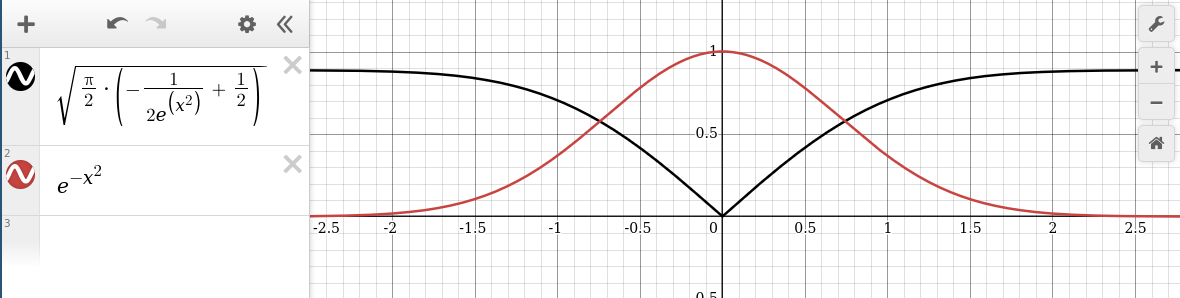
\includegraphics[scale=0.3]{images/3a}\\
        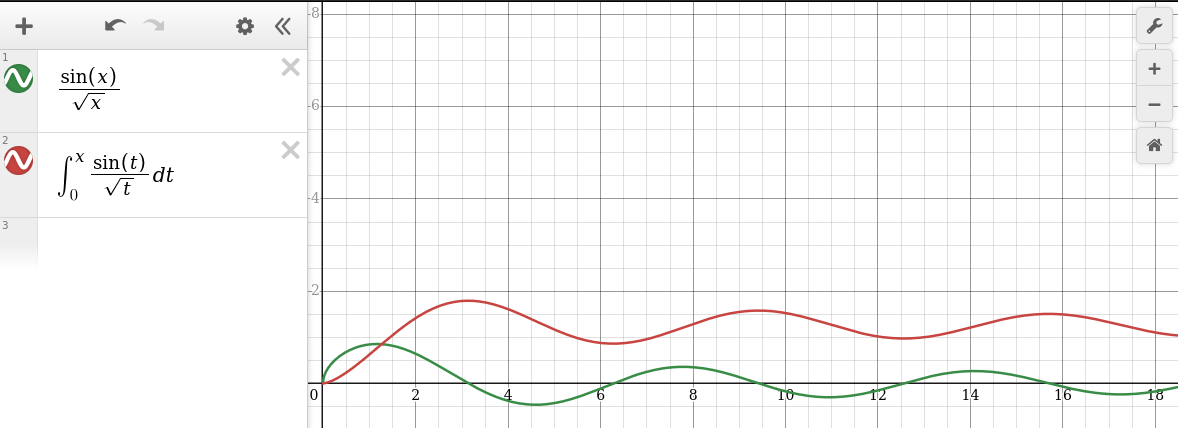
\includegraphics[scale=0.3]{images/3b}\\
        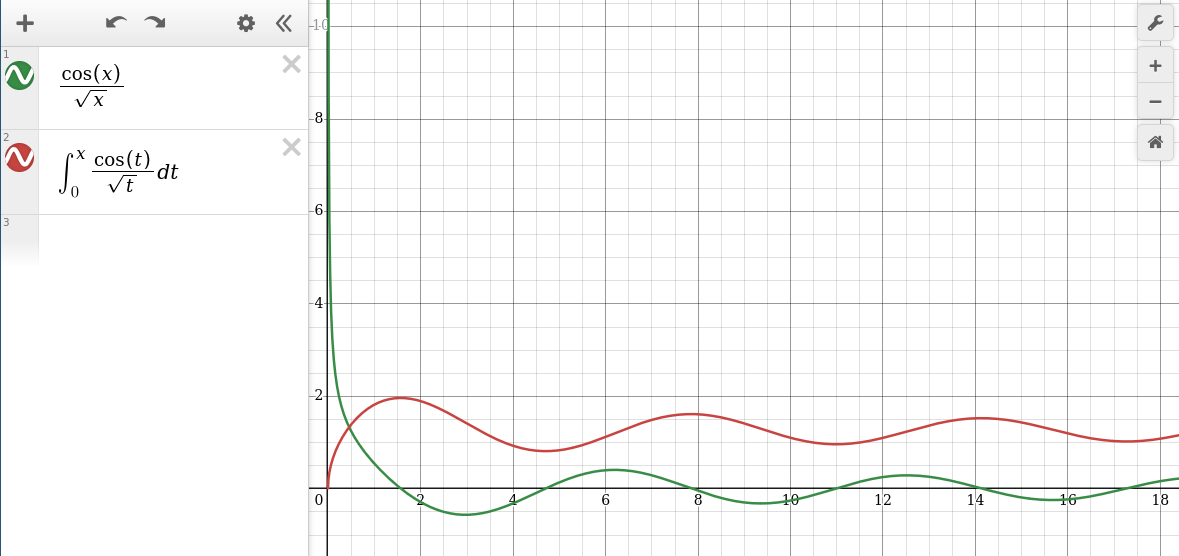
\includegraphics[scale=0.3]{images/3c}\\

\end{enumerate}
\clearpage
